\iffalse
\author{Manvik Muthyapu - AI24BTECH11021}
\section{xe}
\chapter{2010}
\fi

\item[] \textbf{Common Data for Questions 19 and 20:}\\

The velocity field of a two-dimensional fluid flow is as follows:
$$u=U_{0}\frac{x}{L}, v=-U_{0}\frac{y}{L}$$
\text{Where, $U_{0}$ and $L$ are, respectively, the characteristic velocity and length.}

%19
\item  If $L=0.2$m and the resultant of total accelerations in $x$- and $y$- directions at $\brak{x=L ,y=L}$ is $10$m/s$^2$, the magnitude of $U_{0}\brak{\text{m/s}}$ is

\begin{enumerate}
	\item $ 1.414 $
	\item $2.38$
	\item $1.19$
	\item $11.90$
\end{enumerate}

%20
\item The above fluid flow can be described as

\begin{enumerate}
	\item rotational and compressible
	\item irrotational and compressible
	\item rotational and incompressible
	\item irrotational and incompressible\\
\end{enumerate}

\textbf{Linked Answer Questions}\\

\textbf{Statement for Linked Answer Question 21 and 22}\\

The boundary layer formation over a flat plate is shown in the figure below. The variation of horizontal velocity $\brak{u}$ with $y$ at any $x$ along the plate in the boundary layer is approximated as: $u=Psin\brak{Qy}+R$\\

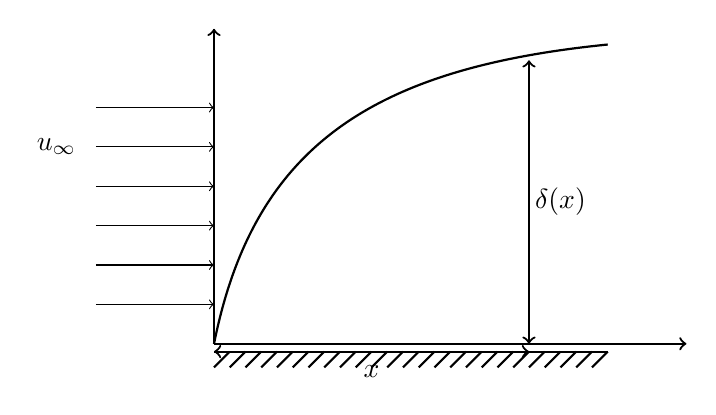
\begin{tikzpicture}

    % Draw axes
    \draw[thick,->] (0,0) -- (6,0);  % x-axis
    \draw[thick,->] (0,0) -- (0,4);  % y-axis
    
    % Draw velocity profile (boundary layer) with a more pronounced curve
    \draw[thick] (0,0) .. controls (0.5,2.5) and (2,3.5) .. (5,3.8);

    % Draw delta(x) with a solid vertical line and double arrows
    \draw[thick,<->] (4,0) -- (4,3.6);  % Extended vertical line up to the curve with double arrows
    \node at (4.4, 1.8) {$\delta(x)$};  % Label for delta(x) moved to the right

    % Draw a horizontal line below the x-axis with double arrows
    \draw[thick,<->] (0,-0.1) -- (4,-0.1);  % Horizontal line below x-axis
    \node at (2,-0.35) {$x$};  % Label for x moved further down

    % Draw arrows representing free-stream velocity
    \foreach \y in {0.5, 1, 1.5, 2, 2.5, 3} {
        \draw[->] (-1.5,\y) -- (0,\y);
    }
    \node at (-2,2.5) {$u_\infty$};

    % Draw the flat plate line
    \draw[thick] (0,-0.1) -- (5,-0.1);

    % Draw inclined lines along the bottom to create a rough surface effect
    \foreach \x in {0.2, 0.4, 0.6, 0.8, 1, 1.2, 1.4, 1.6, 1.8, 2, 2.2, 2.4, 2.6, 2.8, 3, 3.2, 3.4, 3.6, 3.8, 4, 4.2, 4.4, 4.6, 4.8, 5} {
        \draw[thick] (\x,-0.1) -- ++(-0.2,-0.2);
    }

\end{tikzpicture}

%21
\item The most acceptable boundary conditions are

\begin{enumerate}
	\item at $y=0$, $u=0$; at $y=\delta,u=U_{\infty}$ ; at $y=0,\frac{du}{dy} = 0$
	\item at $y=0$, $u=U_{\infty}$; at $y=\delta,u=U_{\infty}$ ; at $y=0,\frac{du}{dy} = 0$
	\item at $y=0$, $u=0$; at $y=\delta,u=U_{\infty}$ ; at $y=\delta,\frac{du}{dy} = 0$
	\item at $y=0$, $u=U_{\infty}$; at $y=\delta,u=U_{\infty}$ ; at $y=\delta,\frac{du}{dy} = 0$
\end{enumerate}

%22
\item Expressions for $P,Q\text{ and }R$ are
	
\begin{enumerate}
	\item $P=0; Q=0; R=0$
	\item $P=U_{\infty}; Q=0; R=0$
	\item $P=0; Q=\frac{\pi}{2\delta}; R=U_{\infty}$
	\item $P=U_{\infty}; Q=\frac{\pi}{2\delta}; R=0$\\
\end{enumerate}

\begin{center}
    \textbf{Useful Data}
\end{center}

\begin{tabular}{@{}l l@{}}
    Avogadro's number & \( : 6.023 \times 10^{23} \ \text{mol}^{-1}\) \\
    Boltzmann's constant \((k_B)\) & \( : 1.38 \times 10^{-23} \ \text{J K}^{-1}\) \\
    Electron charge \((e)\) & \( : 1.602 \times 10^{-19} \ \text{C}\) \\
    Gas Constant & \( : 8.314 \ \text{J mol}^{-1} \ \text{K}^{-1}\) \\
    Electron rest mass & \( : 9.1 \times 10^{-31} \ \text{kg}\) \\
    Permittivity of vacuum \((\varepsilon_0)\) & \( : 8.854 \times 10^{-12} \ \text{F m}^{-1}\) \\
    Planck's constant \((h)\) & \( : 6.626 \times 10^{-34} \ \text{J s}\) \\
    Bohr magneton \((\mu_B)\) & \( : 9.27 \times 10^{-24} \ \text{A m}^2\) \\
    Free space permeability \((\mu_0)\) & \( : 4 \pi \times 10^{-7} \ \text{H m}^{-1}\) \\
    \( 1 \text{J} = 6.242 \times 10^{18} \ \text{eV}\) \\
    \(1 text{eV} = 1.602 \times 10^{-19} \ \text{J}\) \\
    \(1 \text{cal} = 4.2 \ \text{J}\) \\\\
\end{tabular}

%1
\item The number of lattice points in an ideal Perovskite unit cell is

\begin{enumerate}
	\item $1$
	\item $2$
	\item $4$
	\item $5$
\end{enumerate}

%2
\item A Frenkel defect is

\begin{enumerate}
	\item a pair of cation and anion vacancy
	\item a pair of cation interstitial and cation vacancy
	\item a cation vacancy
	\item an anion vacancy
\end{enumerate}

%3 
\item The angle between the line vector of a screw dislocation and the Burgers vector is

\begin{enumerate}
	\item $0$ degrees
	\item $45$ degrees
	\item $60$ degrees
	\item $90$ degrees
\end{enumerate}

%4
\item The addition of a network modifier to silica

\begin{enumerate}
	\item produces vacancies
	\item enchances the network structure
	\item disrupts the network structure
	\item increases the viscosity
\end{enumerate}

%5
\item The best semiconductor material for LED in the visible range is

\begin{enumerate}
	\item Si
	\item Ge
	\item GaAs
	\item GaAs$_{0.6}$P$_{0.4}$
\end{enumerate}

%6
\item A plain carbon steel sample is water-quenched from $900\degree$C to room temperature. Its microstructure will consist of

\begin{enumerate}
	\item pearlite
	\item bainite
	\item martensite
	\item ferrite and pearlite
\end{enumerate}

%7
\item Graphite at zero Kelvin is a

\begin{enumerate}
	\item good conductor
	\item insulator
	\item semiconductor
	\item semi-metal
\end{enumerate}

%8
\item A high molecular weight polyethylene has an average molecular weight of $560,000$g/mol. Its average degree of polymerization is

\begin{enumerate}
	\item $15,000$
	\item $18,660$
	\item $19,310$
	\item $20,000$
\end{enumerate}

%9
\item In which region of the spectra crystal lattice absorption is very significant

\begin{enumerate}
	\item ultraviolet
	\item visible
	\item microwave
	\item infrared
\end{enumerate}

